%-----------------------------------------------------------------------------%
\chapter{\babDua}
%-----------------------------------------------------------------------------%

This chapter focuses on building a conceptual framework by reviewing existing
literature and documentation of the underlying concepts of this research.

%-----------------------------------------------------------------------------%
\section{Web Framework}
%-----------------------------------------------------------------------------%

A web framework is a software framework that is designed to support the
development of web applications. It consists of reusable components that solve
common problems in web application development. Most web frameworks provide
safe defaults to prevent security problems in the web application. This helps
programmers build web applications faster and safer. Some web frameworks also
help maintain better application structure by enforcing software design
patterns.

The common components of a web framework are the dispatcher, the decoder, the
generator, and the store \cite{schwarz_webframework}. The dispatcher maps
Uniform Resource Locators (URLs) to application code that is invoked when an
HTTP request is received. The decoder decodes the client request, which allows
the web application to read parameters, headers, and request body data sent as
part of the request. The generator constructs the output that is sent as a
response to the client. The store holds inter-request data, which is usually
stored in a database system.

%-----------------------------------------------------------------------------%
\section{Django and Object-Relational Mapping}
%-----------------------------------------------------------------------------%

Django is a free and open-source web framework written in Python \cite{django}.
Its overall philosophies are loose coupling, less code, quick development,
don't repeat yourself (DRY), explicit is better than implicit, and consistency
\cite{django:philosophies}. It follows what it calls the model-template-view
architectural pattern, which shares similarities to the model-view-controller
pattern \cite{django:faq}. It consists of an object-relational mapping (ORM)
system that handles the interaction with database systems, a template system
that defines how the data looks like to the user, and a view system that
defines which data is presented to the user.

Object-relational mapping (ORM) is a programming technique that allows its
users to query and manipulate data stored in a relational database using an
object-oriented paradigm \cite{linskey:orm}. Object query, load, and delete
operations are translated into SQL SELECT and DELETE statements, while object
allocation and modification operations are translated into SQL INSERT and
UPDATE statements. To achieve this, the scalar values retrieved from the
database are converted into object instances in the program and vice versa.

The ORM system in Django maps data models to relational database tables. The
data models are represented as Python classes. The model class also has
attributes, called model fields, which represent the columns of the database
table. These model fields define the data types that are used in the database.
For example, the CharField model field uses the VARCHAR data type in the
database. In addition, these model fields also define the behavior of the
columns, such as their NOT NULL and UNIQUE constraints in the database.

Aside from storing and loading data, the ORM system in Django also provides
querying capabilities through the use of lookups and transforms. Lookups and
transforms are specified using keyword arguments in the form of
\code{field\_\_lookuptype=value}, where \code{lookuptype} can be a lookup or
transform name. Lookups define how the WHERE clause of an SQL query is composed
by Django. Transforms are used to transform a model field from one form to
another (e.g. extracting the year from a DateField). For example, a query
specified in Python as shown in \autoref{code:query1py} will be translated into
an SQL query equivalent shown in \autoref{code:query1sql}.

\lstinputlisting[
	language=Python,
	caption={
		A query on a DateField named \code{pub\_date}
		with the \code{year} transform and \code{gte} lookup.},
	label=code:query1py]{codes/2-query1.py}

\lstinputlisting[
	language=SQL,
	caption={An SQL query equivalent to \autoref{code:query1py}.},
	label=code:query1sql]{codes/2-query1.sql}

Django officially supports five database backends: PostgreSQL, MariaDB, MySQL,
SQLite, and Oracle Database \cite{django:databases}. Each database backend
(other than SQLite) requires a compatible database driver to be installed. The
database backends provided by Django adapt the database drivers so that they
can be used with the ORM system. These backends are implemented in the
django.db.backends module.

%-----------------------------------------------------------------------------%
\section{JSON in Relational Database Systems Supported by Django}
%-----------------------------------------------------------------------------%

JavaScript Object Notation (JSON) is a lightweight, text-based data-interchange
format \cite{json}. It is designed to be human-readable and easy for machines
to parse and generate. It is based on a subset of the JavaScript standard, but
it is completely language independent. It uses conventions that are similar to
popular programming languages such as C, C++, C\#, Java, JavaScript, Python,
and many others. These properties make JSON a widely-used data-interchange
format, especially in web applications.

JSON is built on two structures: an unordered set of key-value pairs (called
JSON objects) and an ordered list of values (called JSON arrays). The values
can be scalar values such as strings, numbers, booleans, or null. However, they
can also be JSON objects or JSON arrays, which means that they can be nested
to form more complex data structures. An example of a JSON object that contains
a JSON array and other JSON objects can be seen in \autoref{code:json}.

\lstinputlisting[
	language=Python,
	caption=A JSON object that contains a JSON array and other JSON objects.,
	label=code:json]{codes/2-json.json}

To utilize the flexibility of JSON, some relational databases have implemented
support for storing and querying JSON data. This is commonly done by providing
database functions to operate on JSON data stored as text or, in some cases, a
native JSON data type. JSON support on the database systems supported by Django
varies between one another. This section explains how those database systems
provide JSON support.

\subsection{PostgreSQL}

PostgreSQL supports a native JSON data type and JSON functions as of version
9.2 \cite{postgresql:9.2}. Data stored using the JSON data type is stored as
text. However, it has the advantage of validating that each stored value is
valid JSON. The two JSON functions included in the 9.2 release allow users to
convert a row or array in the database into JSON.

As of version 9.4, PostgreSQL also supports a JSONB data type and more JSON
functions \cite{postgresql:9.4}. JSONB supports fast data retrievals and simple
expression search queries using Generalized Inverted Indexes (GIN). Data stored
using the JSONB data type is stored as binary. This makes storing data with the
JSONB data type is slightly slower compared to the JSON data type as it needs
to be encoded into binary prior to saving. However, it is significantly faster
to process, since the processing functions do not need to reparse the data on
each execution. The JSON functions introduced in the 9.4 release enable users
to extract and manipulate JSON data with a performance that matches or
surpasses document databases.

\subsection{MariaDB and MySQL}

MariaDB is highly compatible with MySQL, albeit with some behavior differences
\cite{mariadb:compatibility}. MariaDB is originally designed to be a completely
open-source drop-in replacement for MySQL. MariaDB's client protocol is binary
compatible with MySQL's client protocol, therefore Django uses the same
database backend for MySQL and MariaDB \cite{django:databases}. Both database
systems have compatible JSON functions to operate on JSON data, but the data
is stored differently.

MySQL supports a native JSON data type as of version 5.7.8 \cite{mysql:json}.
The JSON data type provides automatic validation of JSON data. It is internally
stored as binary, which permits quick read access as the value does not need to
be parsed from a text representation. Data stored using the JSON data type can
be indexed by using a generated column that extracts a scalar value from the
JSON data.

MariaDB has a JSON data type as of version 10.2.7 \cite{mariadb:json}. The JSON
data type was introduced for compatibility reasons with MySQL's JSON data type.
However, this JSON data is an alias for the LONGTEXT data type. Despite the
data is stored as a string rather than binary, it can be validated using the
provided JSON\_VALID function as a CHECK constraint.

\subsection{SQLite}

SQLite has the JSON1 extension as of version 3.9.0 \cite{sqlite:3.9.0}. The
JSON1 extension is a loadable extension that includes functions that can be
used to manage JSON content \cite{sqlite:json1}. As of this writing, the JSON1
extension stores JSON data as text. JSON data can be validated using the
included JSON\_VALID function as a CHECK constraint.

\subsection{Oracle Database}

Oracle Database supports storing, validating, querying, and indexing JSON data
as of version 12.1.0.2 \cite{oracle:12.1.0.2}. JSON data is stored using SQL
data types VARCHAR2, CLOB, and BLOB \cite{oracle:json}. JSON validation can be
enforced using the IS JSON condition as a CHECK constraint. Querying JSON data
can be performed by utilizing the provided JSON functions. Indexing JSON data
can be implemented using bitmap, function-based, or composite B-tree indexes.

%-----------------------------------------------------------------------------%
\section{Keterkaitan Teori Dengan Penelitian}
%-----------------------------------------------------------------------------%
\todo{Ada baiknya setelah menjelaskan teori-teori, Anda menjelaskan apa kaitan teori tersebut dengan penelitian Anda. Hal ini tentunya membantu pembaca dalam memahami bahwa teori yang Anda paparkan memang penting untuk memahami penelitian Anda nantinya.}

\begin{figure}
	\centering
	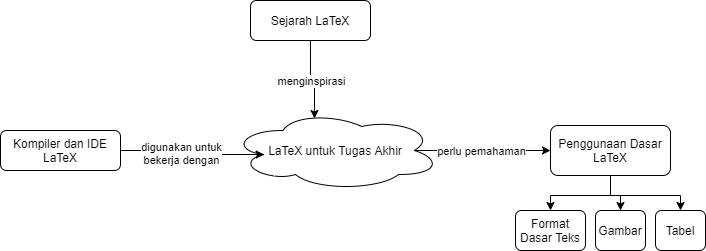
\includegraphics[width=\textwidth]{pics/research_concept_map.png}
	\caption{Keterkaitan konsep hasil studi literatur terhadap penelitian}
	\label{fig:research_concept_map}
\end{figure}

\todo{Jelaskan \pic~\ref{fig:research_concept_map} di sini. Setiap gambar pada
tugas akhir butuh penjelasan. Gambar hadir untuk mempermudah membaca memahami
konteks, tetapi tidak bisa berdiri sendiri tanpa penjelasan. Terkait gambar,
Anda juga bisa mengatur skalanya. Gambar kali ini lebarnya 0,8x dari lebar teks
halaman.}
